\subsection{\Bhh Normalisation}
\label{subsubsec:BhhNormalisation}

To get a realistic measurement of the \Bd signal yield, which could otherwise be unrealistically inflated (or deflated) by the \Bhh and \Bdmumu invariant mass overlap when fitted to data, the \Bhh normalisation will be externally constrained in the final fit to data and hence a realistic estimate of the resonant background yield is required.

SM predicted estimates can be calculated by considering the \Bhh equivalent of the master euqation~\ref{eq:BRFormula}, rearranged for the dimuon yield and using the latest measurements of the \Bhh branching ratios from PDG \cite{ParticleDataGroup:2024cfk}. Such predictions have been calculated by incorporating the the estimated \Bpm  yield of Chapter~\ref{sec:ReferenceChannel}, ratio of acceptance times efficiency from Chapter~\ref{sec:AccepEffRatio}, and using the fake rates from Chapter~\ref{sec:FakeBackground} \textcolor{red}{Dont forget to update these chapters to sections where the numbers are. For now PR2 fakes rates are being used}.

\DJcomment{Table~\ref{tab:MasterEqEstMuonWPs} shows the SM predictions for \Bmumu and \Bhh yields for all combinations of Tight (T) and Loose (L) muons in the final states.}{Why are LNT-T and T-LNT exactly the same for the signals but not Bhh?} 
By construction the Loose but Not Tight (LNT) muons pass the L muon WP but fail the T muon WP, and are therefore orthogonal to the T muons. With two muons in the final state, any combination of L-L, LNT-LNT, LNT-T or T-LNT are orthogonal regions to the T-T region and to each other, and can therefore be used in a fit to data of such regions to extract the \Bhh yield without unblinding and for validation of the full yield extraction procedure.

\begin{table}[h]
  \centering
  \footnotesize
    \begin{tabular}{cccc}
        \toprule
        Region & \Bsmumu & \Bdmumu & \Bhh \\
        \midrule
        LNT-LNT & $4.03 \pm 0.39$ & $0.431 \pm 0.038$ & $21.0 \pm 5.5$ \\ 
        LNT-T & $36.9 \pm 3.5$ & $3.94 \pm 0.34$ & $14.9 \pm 4.2$ \\ 
        T-LNT & $36.9 \pm 3.5$ & $3.94 \pm 0.34$ & $15.7 \pm 4.4$ \\ 
        T-T & $337 \pm 32$ & $36.1 \pm 3.1$ & $13.39 \pm 0.56$ \\ 
        \bottomrule
  \end{tabular}
    \caption{Estimated yields of \Bmumu and \Bhh events for Tight and Loose muon identification requirements based on muon efficiencies and hadron fake rates from MC simulation. 
  \textcolor{red}{Currently these estimates use the intermediate SES\_d from ReA and Njpsi that is a sum of independent fits to individual data periods. Will have to update with proper numbers.}}
  \label{tab:MasterEqEstMuonWPs}
\end{table}

Based upon these yields, we fit the LNT-LNT data region with the adjusted version of the baseline model described in section~\ref{subsec:FitConfig}. The LNT-LNT region provides the best environment to extract the \Bhh yield due to its higher fraction of events with respect to the \Bs and \Bd than the LNT-T or the T-LNT regions. The adjustments to the fit model include:
\begin{itemize}
\item Fixing the \Bs (\Bd) model parameters to the result of the simultaneous extended unbinned maximum likelihood fit in the LNT-LNT region \Bs (\Bd) MC sample to get a more suitable representation of the signal shape in this orthogonal to the signal region,
\item Fixing the \Bhh shape parameters to the result of the corrected LNT-LNT \Bhh MC fit in Chapter~\ref{sec:FakeBackground} \textcolor{red}{change this to the actual section once written},
\item Fixing the non-resonant background model parameters to the result of the data sidebands fit in the T-T region in section~\ref{subsubsec:SimultaneousSSSVplusCOMBcombinedFitMCandDataSB},
\item Leaving the non-resonant background components normalisations free,
\item Fixing the signal yields to the simulation-based master equation estimates of table~\ref{tab:MasterEqEstMuonWPs}

\end{itemize}

The fit quality for low statistic cases, like the LNT-LNT data fit, is evaluated using a different statistic than the Pearson $\chi^2$, which breaks down at low event counts where the $\chi^{2}$ distribution approximation no longer holds. Instead, the Baker-Cousins $\chi^{2}$ ($\chi^{2}_{BC}$) statistic is used since it incorporates the exact Poisson likelihood and hence can accomodate the low statistics Poisson regime. However, the $\chi^{2}_{BC}$ does not follow standard $\chi^{2}$ distribution with a well defined number of degrees of freedom so analytical methods of approximating the p-value with this test statistic are unsuitable. Instead we resort to the frequentist toy MC based approach in calculation of the p-value. The p-value for the goodness of fit is calculated as the fraction of toy MC datasets generated according to the fitted model that provide a $\chi^{2}_{BC}$ that is higher than or equal to the one observed in the fit to the original dataset. This method will hence forth be used in the goodness of fit p-value evaluations of low statistic sample fits due to its reliability in such regimes.

Figure~\ref{fig:LNT-LNTdatafit} shows the result of the LNT-LNT data fit with the adjusted model described earlier in thi section. Visually, the fitted shape reproduces the data well and with a reasonable fit quality in each BDT bin. The goodness of fit was evaluated using the $\chi^{2}_{BC}$, and provides satisfactory p-values in each of the BDT bins. The resulting \Bhh yield was found to be $N^{LNT-LNT}_{hh'} = 13.6 \pm 5.5$ ($21.0 \pm 5.5$ expected) events in the LNT-LNT region.
\begin{figure}[ht!]
  \centering
  \subfloat[BDT bin 0 fit with BDT boundaries at {[0.1609,0.2636]}.]{
    %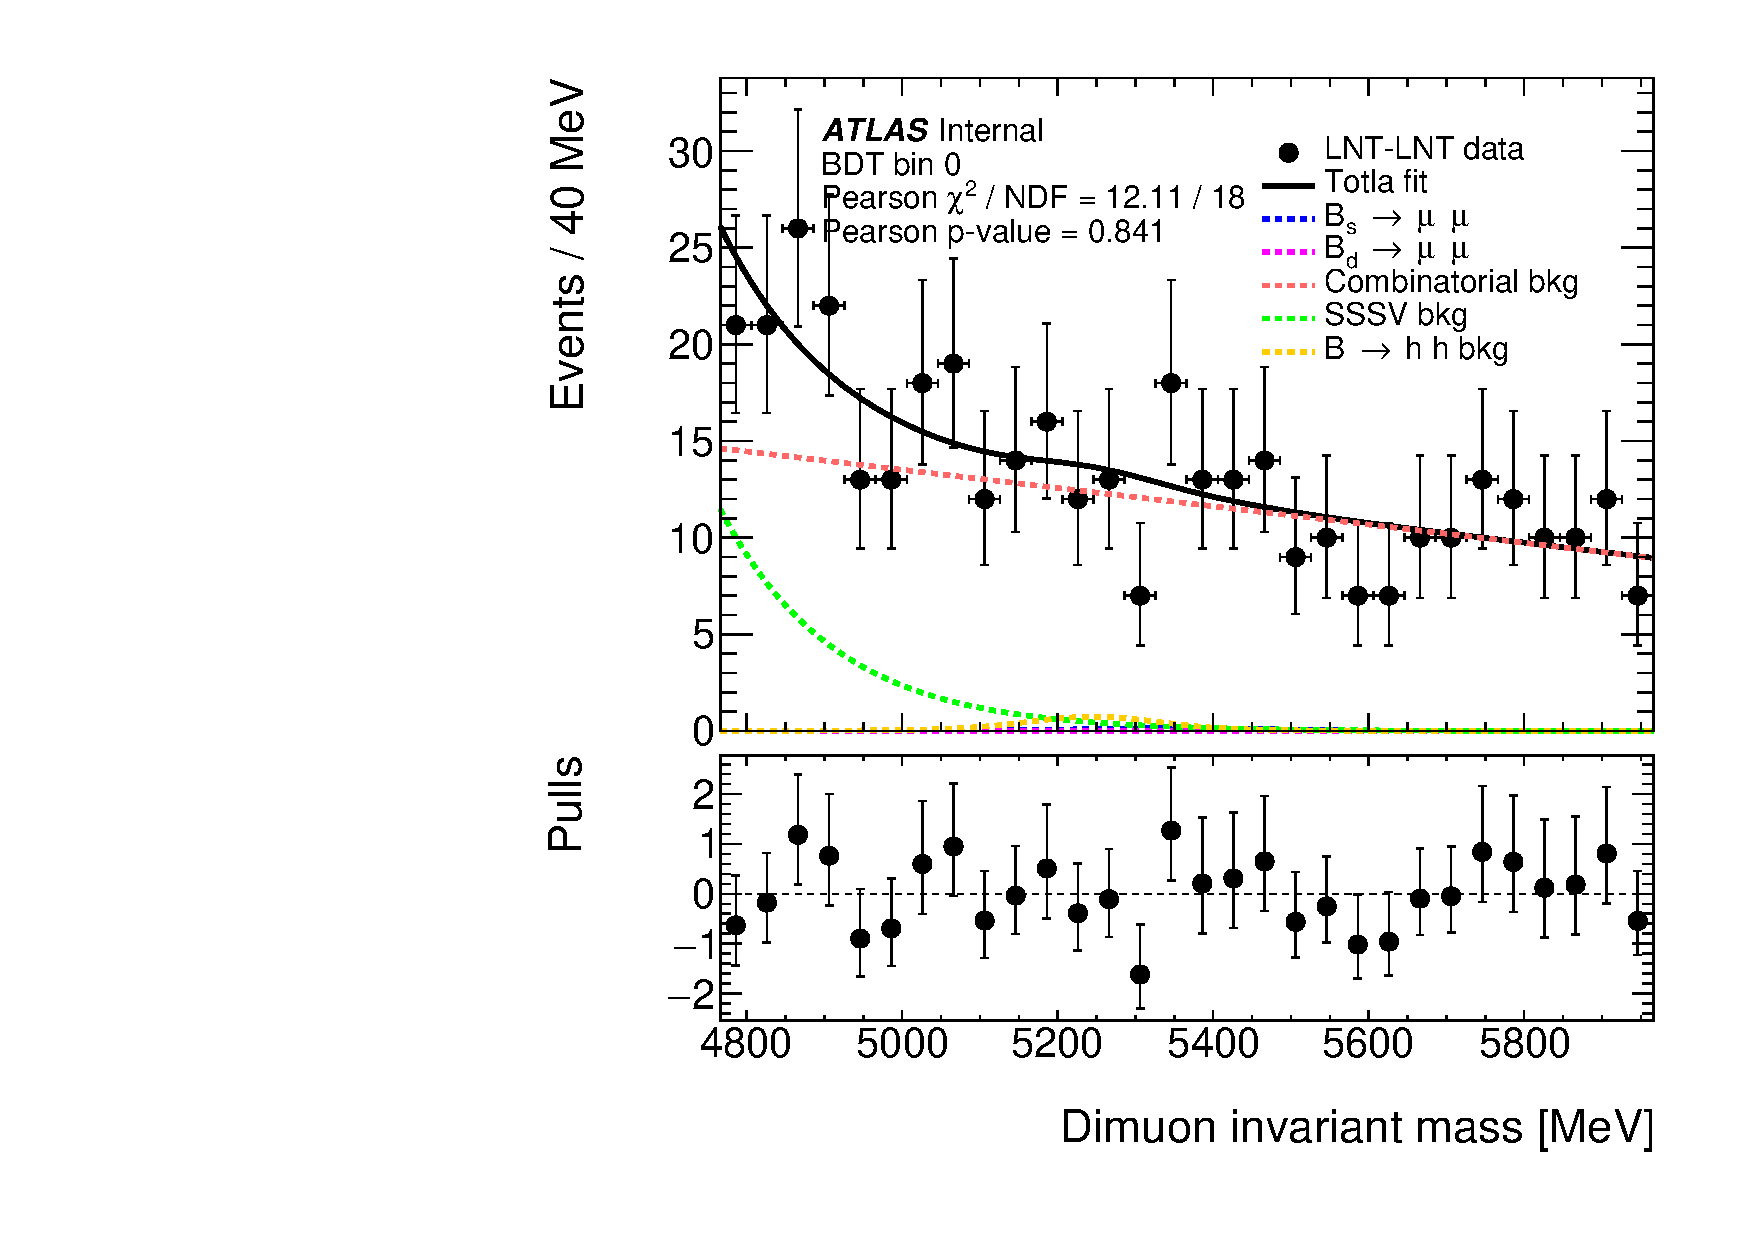
\includegraphics[width=0.5\textwidth]{figures/SignalExtraction/out_fit_Bhh_Bs_Bd_LNT-LNT_Bhh_json_all_other_T-T_nBs_nBd_fixed_pos_def_can_LNT-LNT_BDT_1_ETA_1.pdf}  % p-value from Pearson Chi2 
    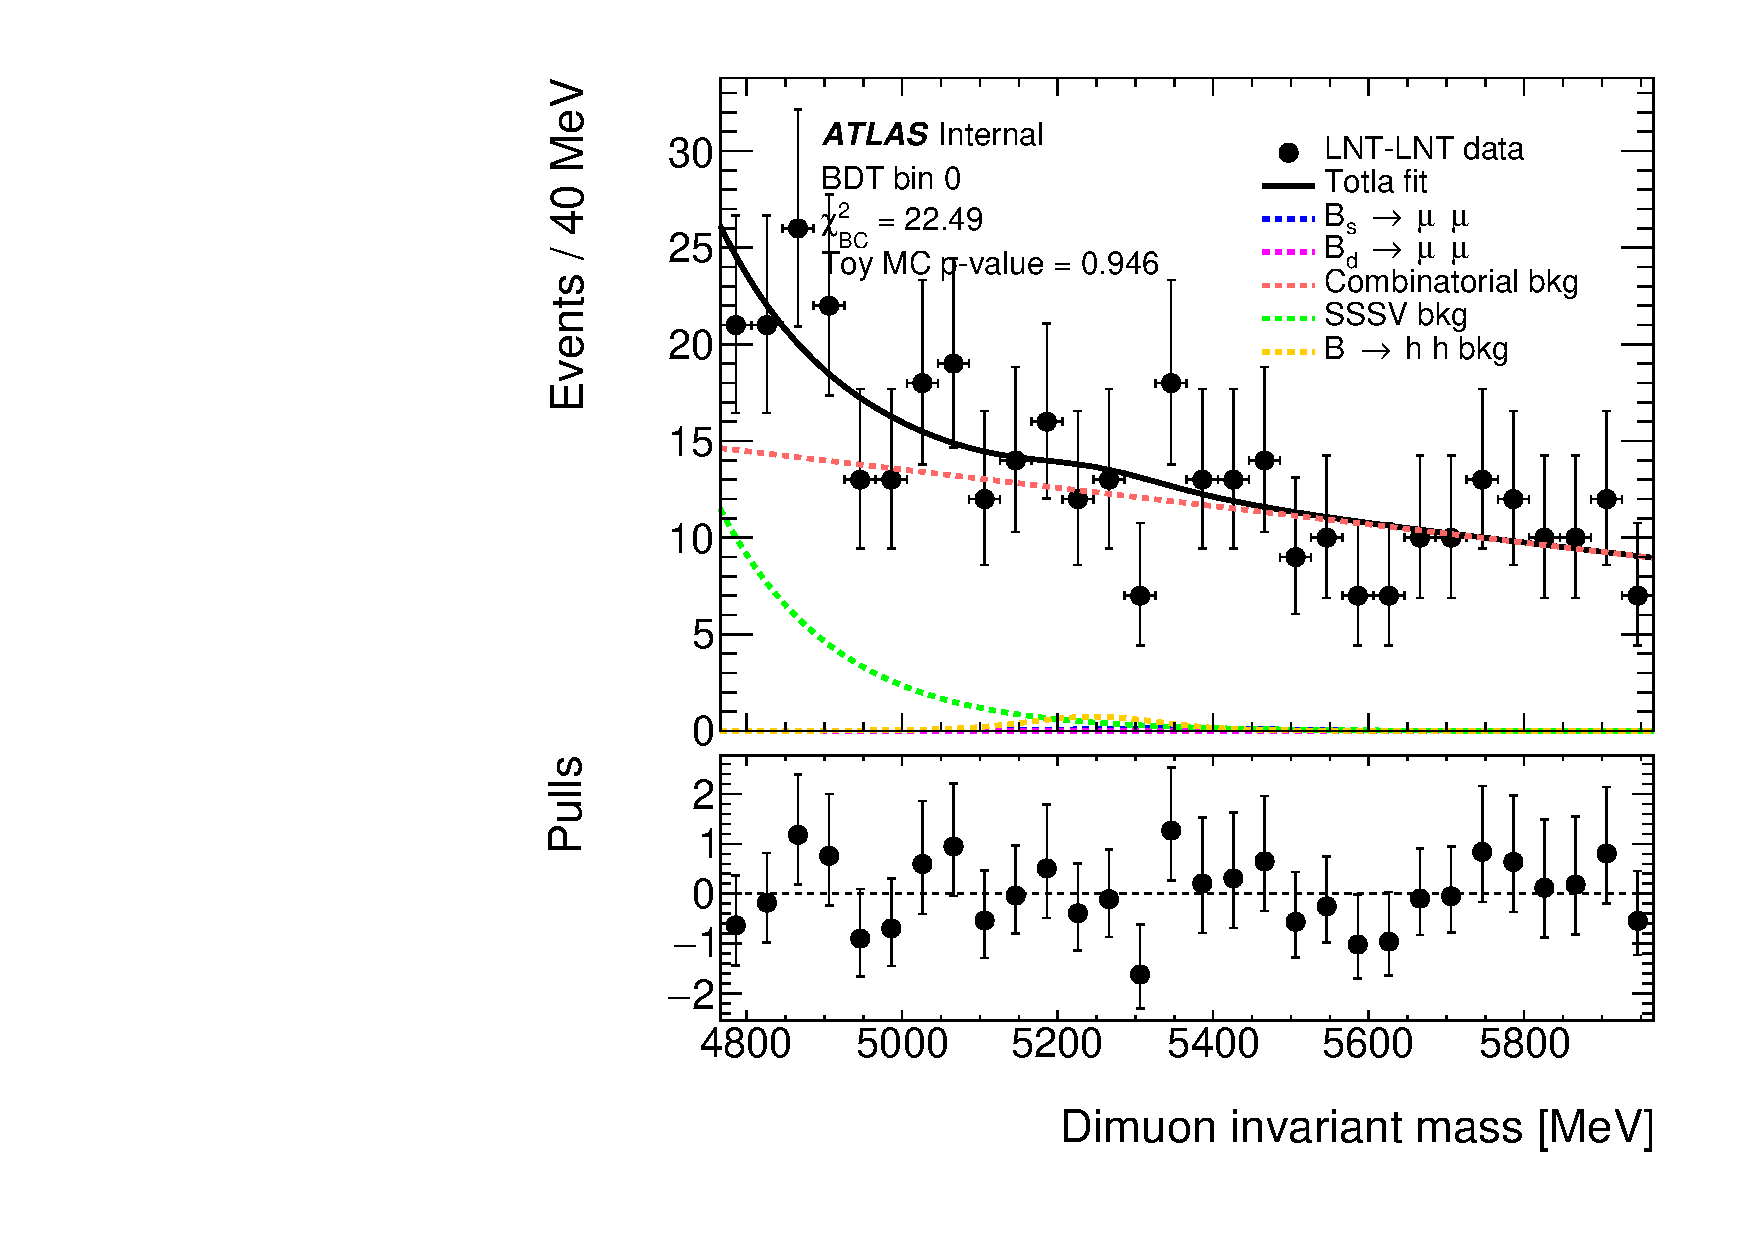
\includegraphics[width=0.5\textwidth]{figures/SignalExtraction/out_fit_Bhh_LNT_LNT_toy_MC_p_val_can_LNT-LNT_BDT_1_ETA_1.pdf}  % p-value from toy MC , BC Chi2 
    \label{fig:LNT-LNTdatafitBin0}
  }
  \subfloat[BDT bin 1 fit with BDT boundaries at {[0.2636,0.3405]}.]{
    %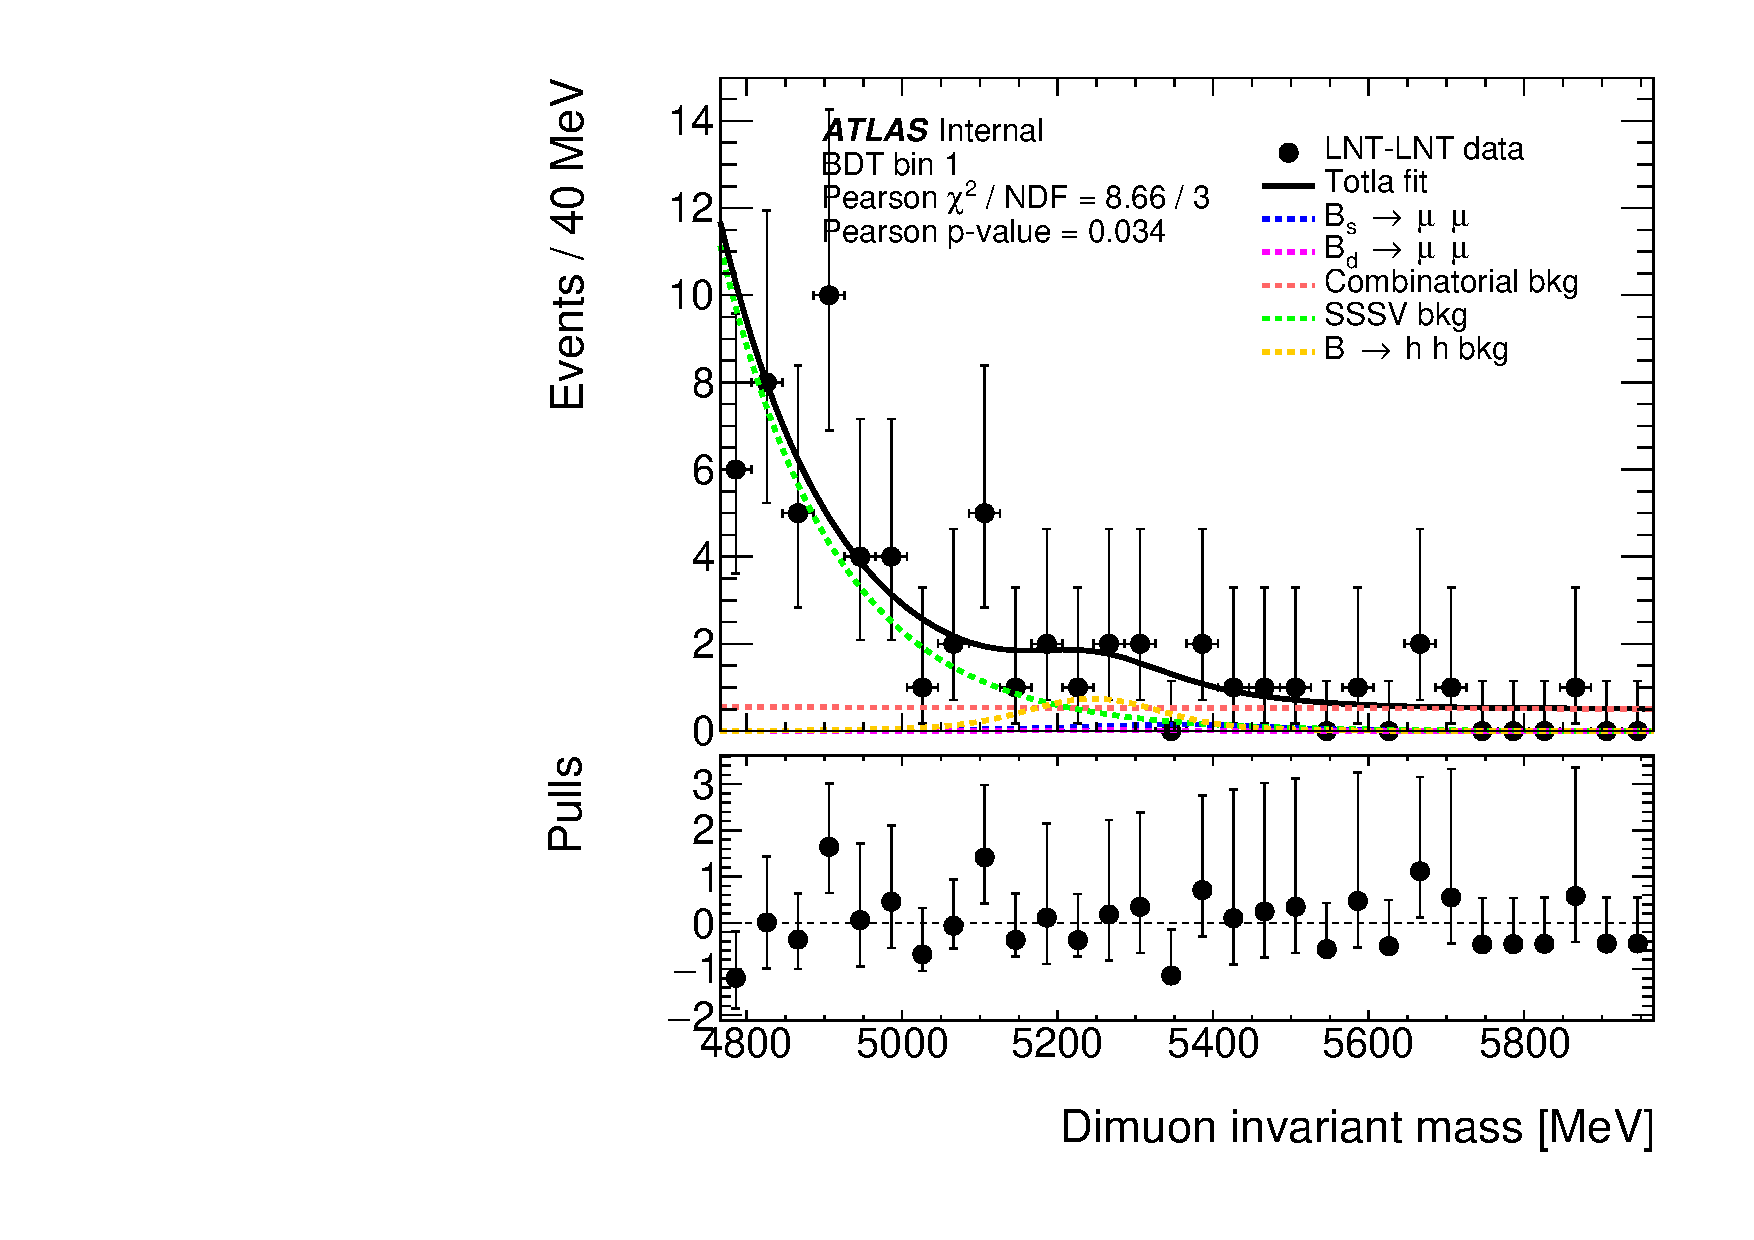
\includegraphics[width=0.5\textwidth]{figures/SignalExtraction/out_fit_Bhh_Bs_Bd_LNT-LNT_Bhh_json_all_other_T-T_nBs_nBd_fixed_pos_def_can_LNT-LNT_BDT_2_ETA_1.pdf}
    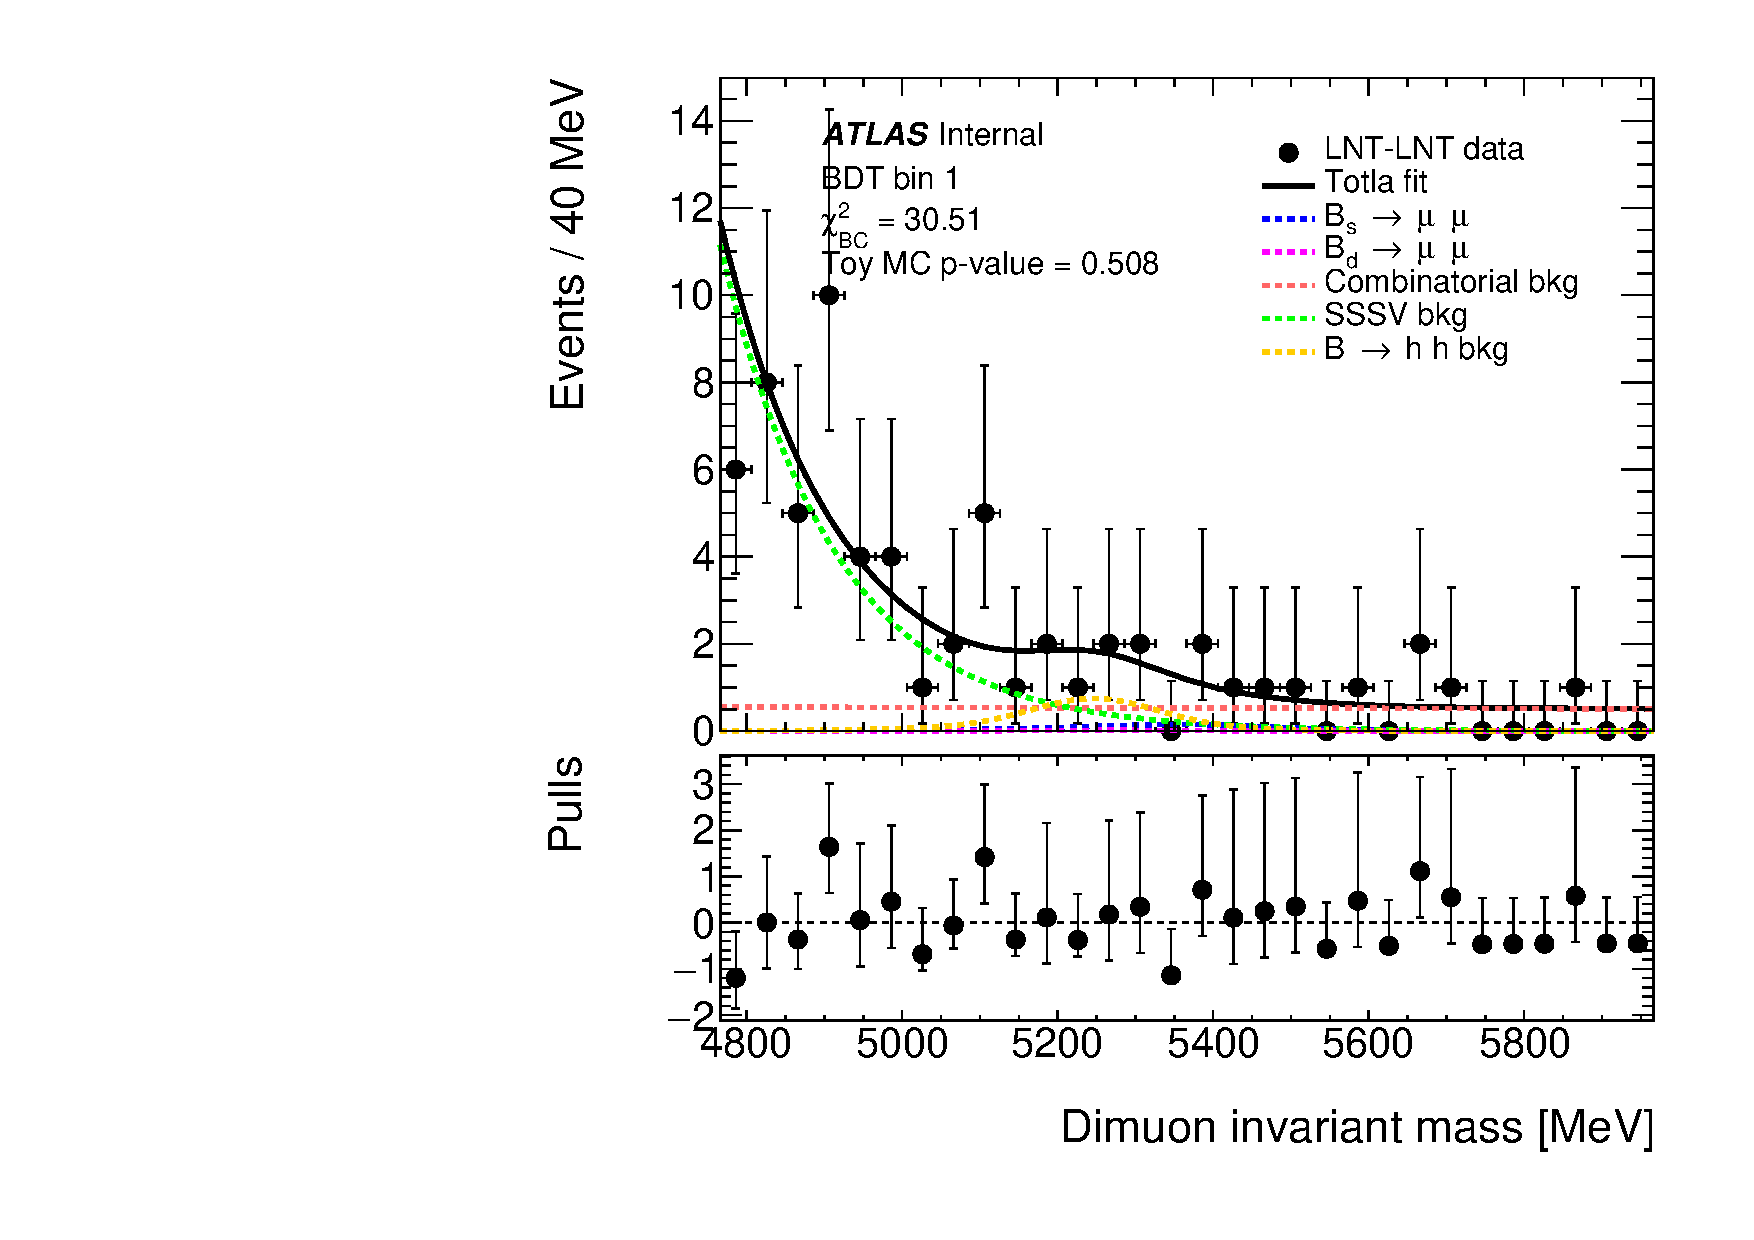
\includegraphics[width=0.5\textwidth]{figures/SignalExtraction/out_fit_Bhh_LNT_LNT_toy_MC_p_val_can_LNT-LNT_BDT_2_ETA_1.pdf}  % p-value from toy MC , BC Chi2 
    \label{fig:LNT-LNTdatafitBin1}
  }
  \\
  \subfloat[BDT bin 2 fit with BDT boundaries at {[0.3405,0.4055]}.]{
    %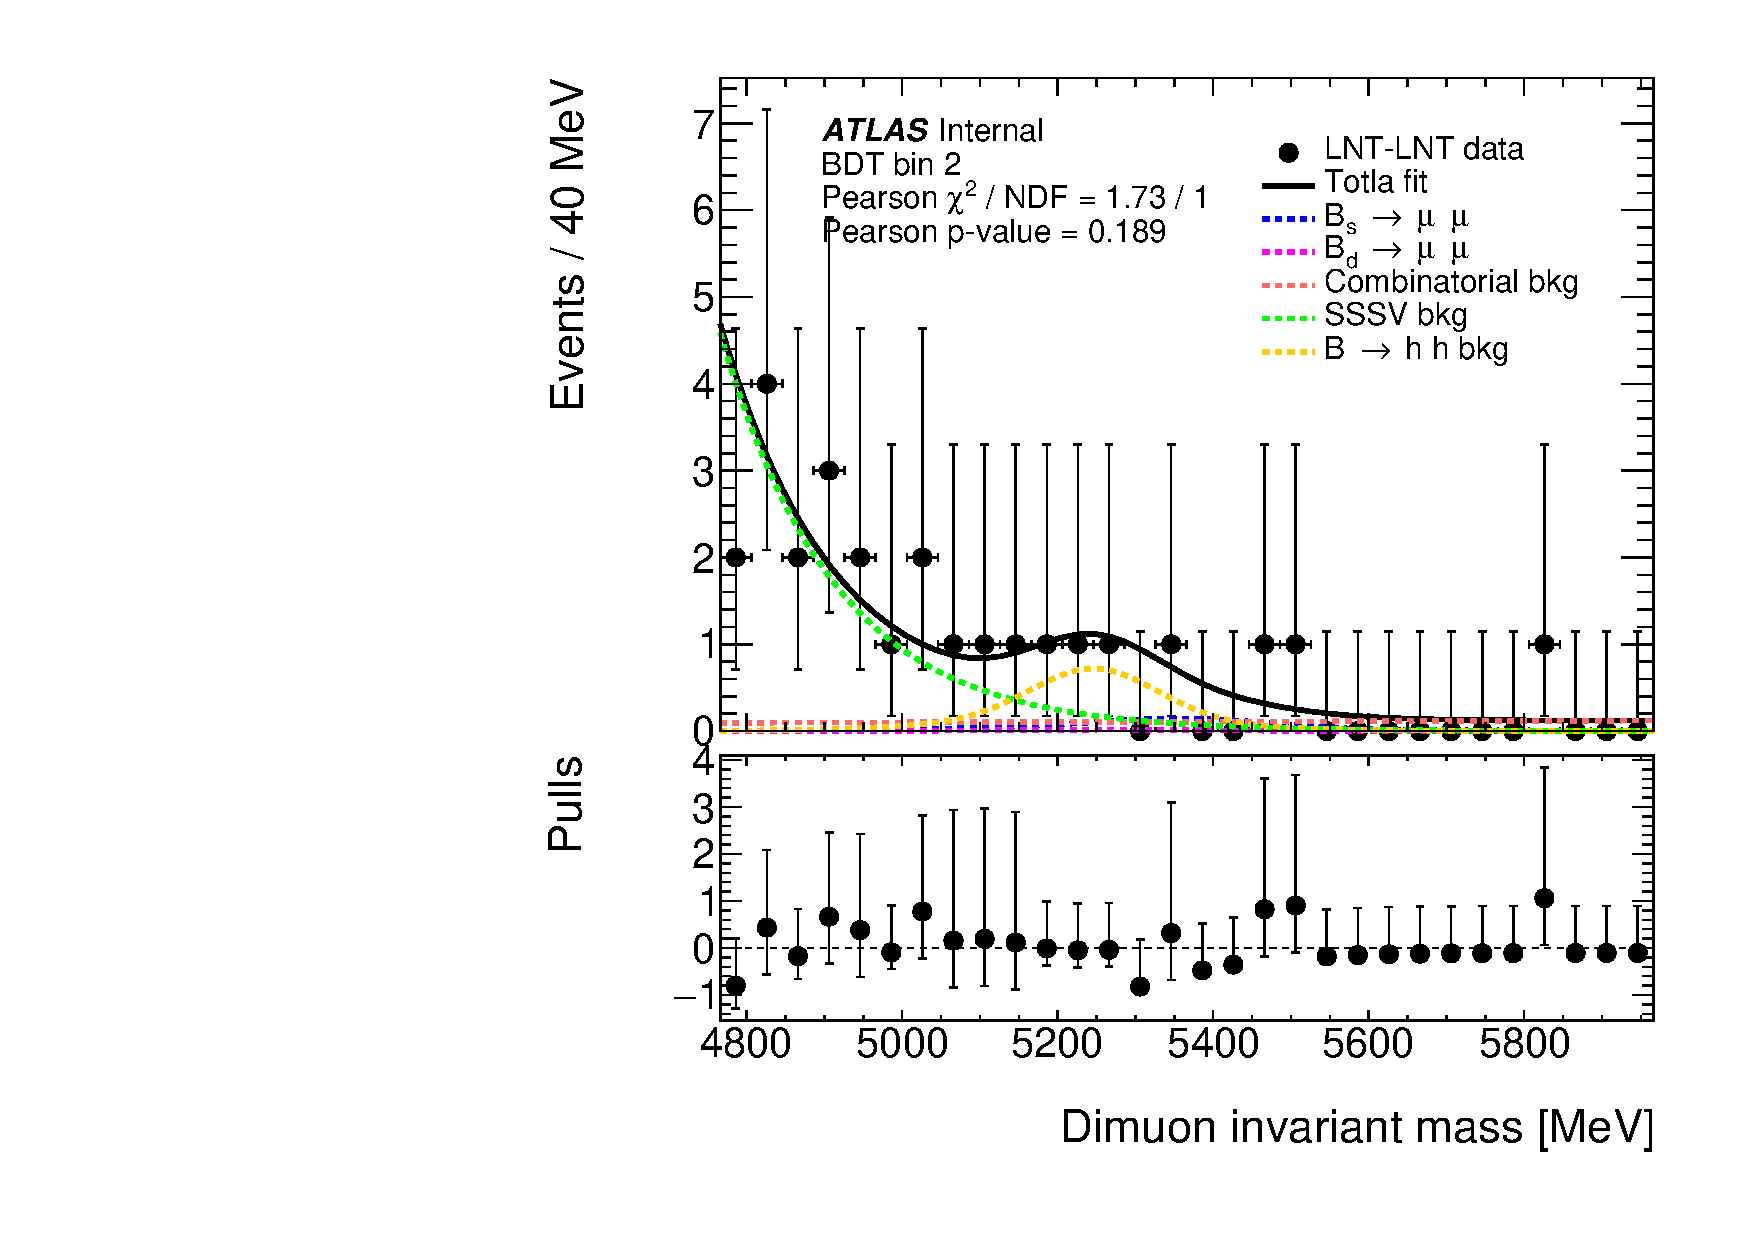
\includegraphics[width=0.5\textwidth]{figures/SignalExtraction/out_fit_Bhh_Bs_Bd_LNT-LNT_Bhh_json_all_other_T-T_nBs_nBd_fixed_pos_def_can_LNT-LNT_BDT_3_ETA_1.pdf}
    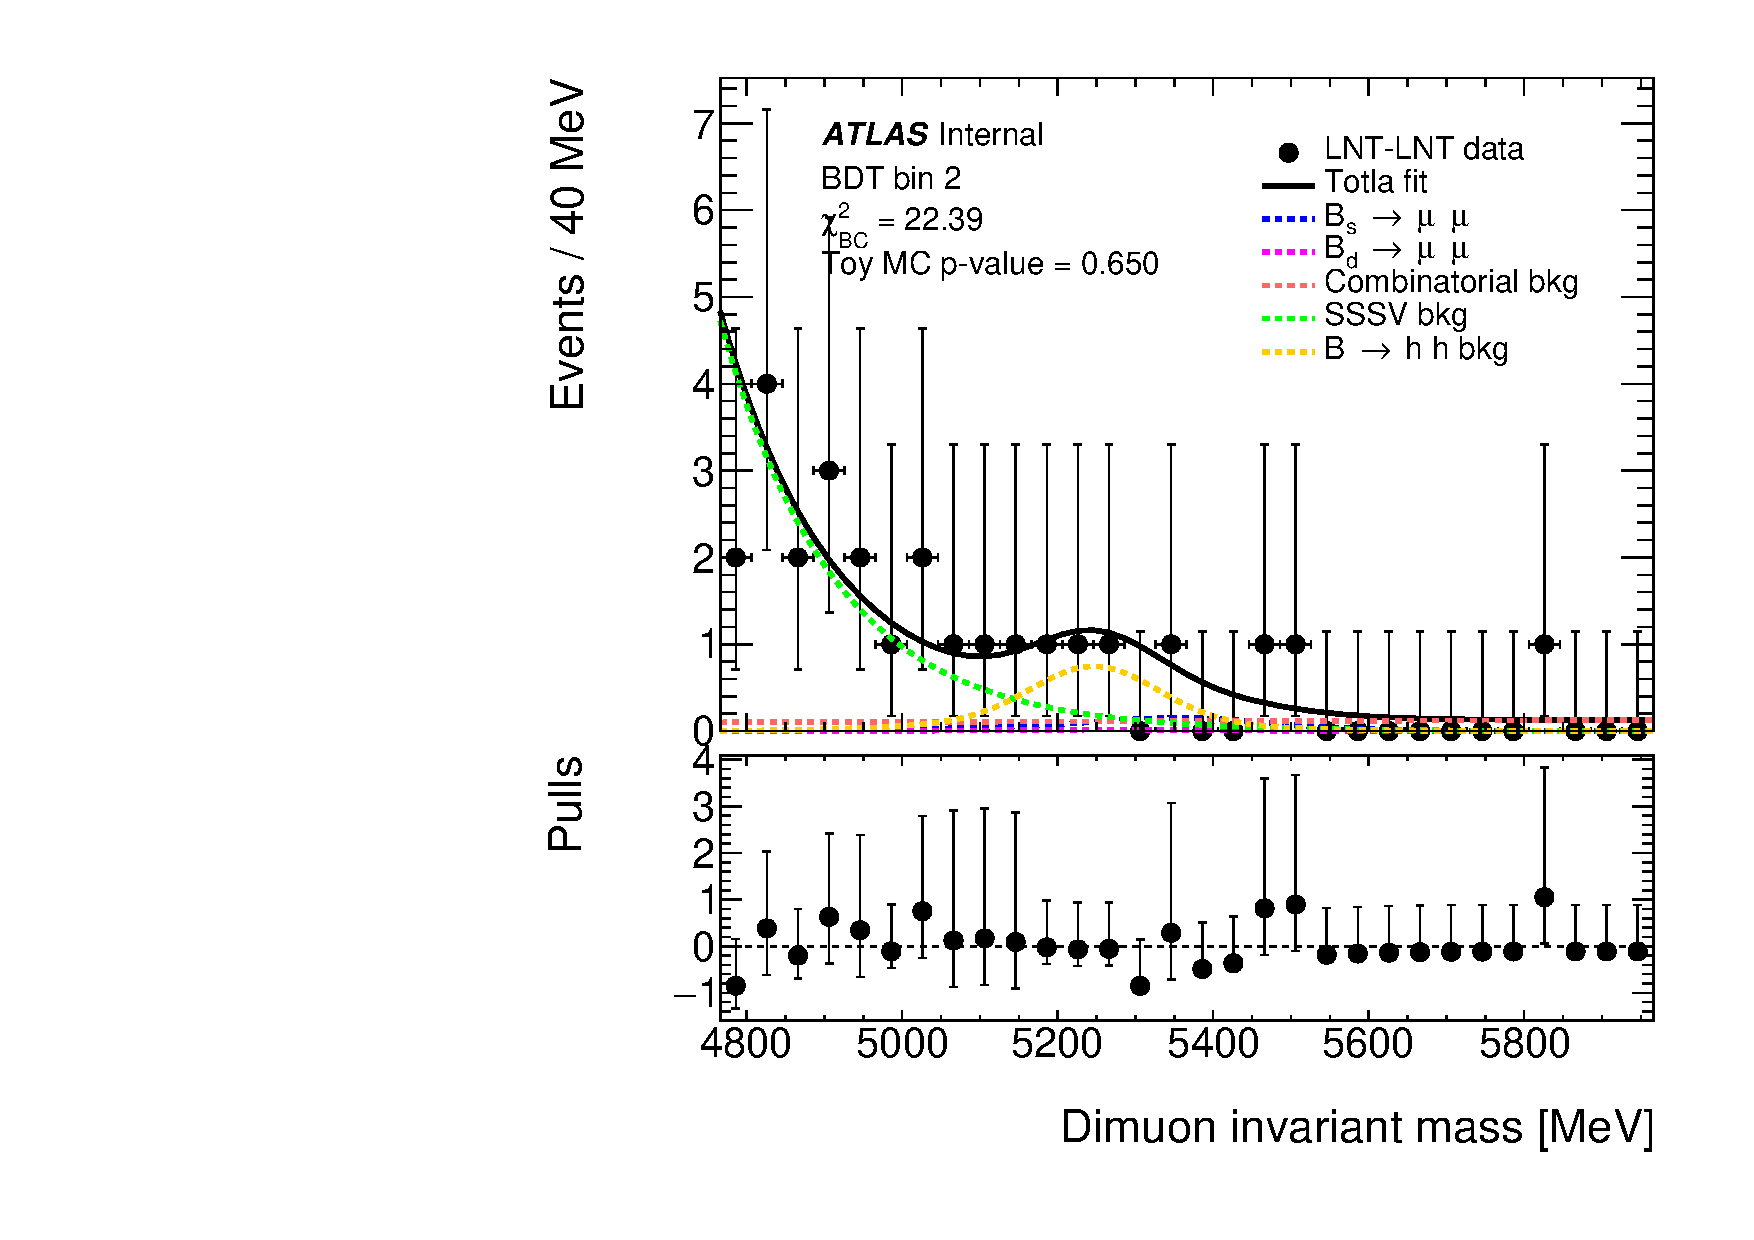
\includegraphics[width=0.5\textwidth]{figures/SignalExtraction/out_fit_Bhh_LNT_LNT_toy_MC_p_val_can_LNT-LNT_BDT_3_ETA_1.pdf}  % p-value from toy MC , BC Chi2 
    \label{fig:LNT-LNTdatafitBin2}
  }
  \subfloat[BDT bin 3 fit with BDT boundaries at {[0.4055,1.0000]}.]{
    %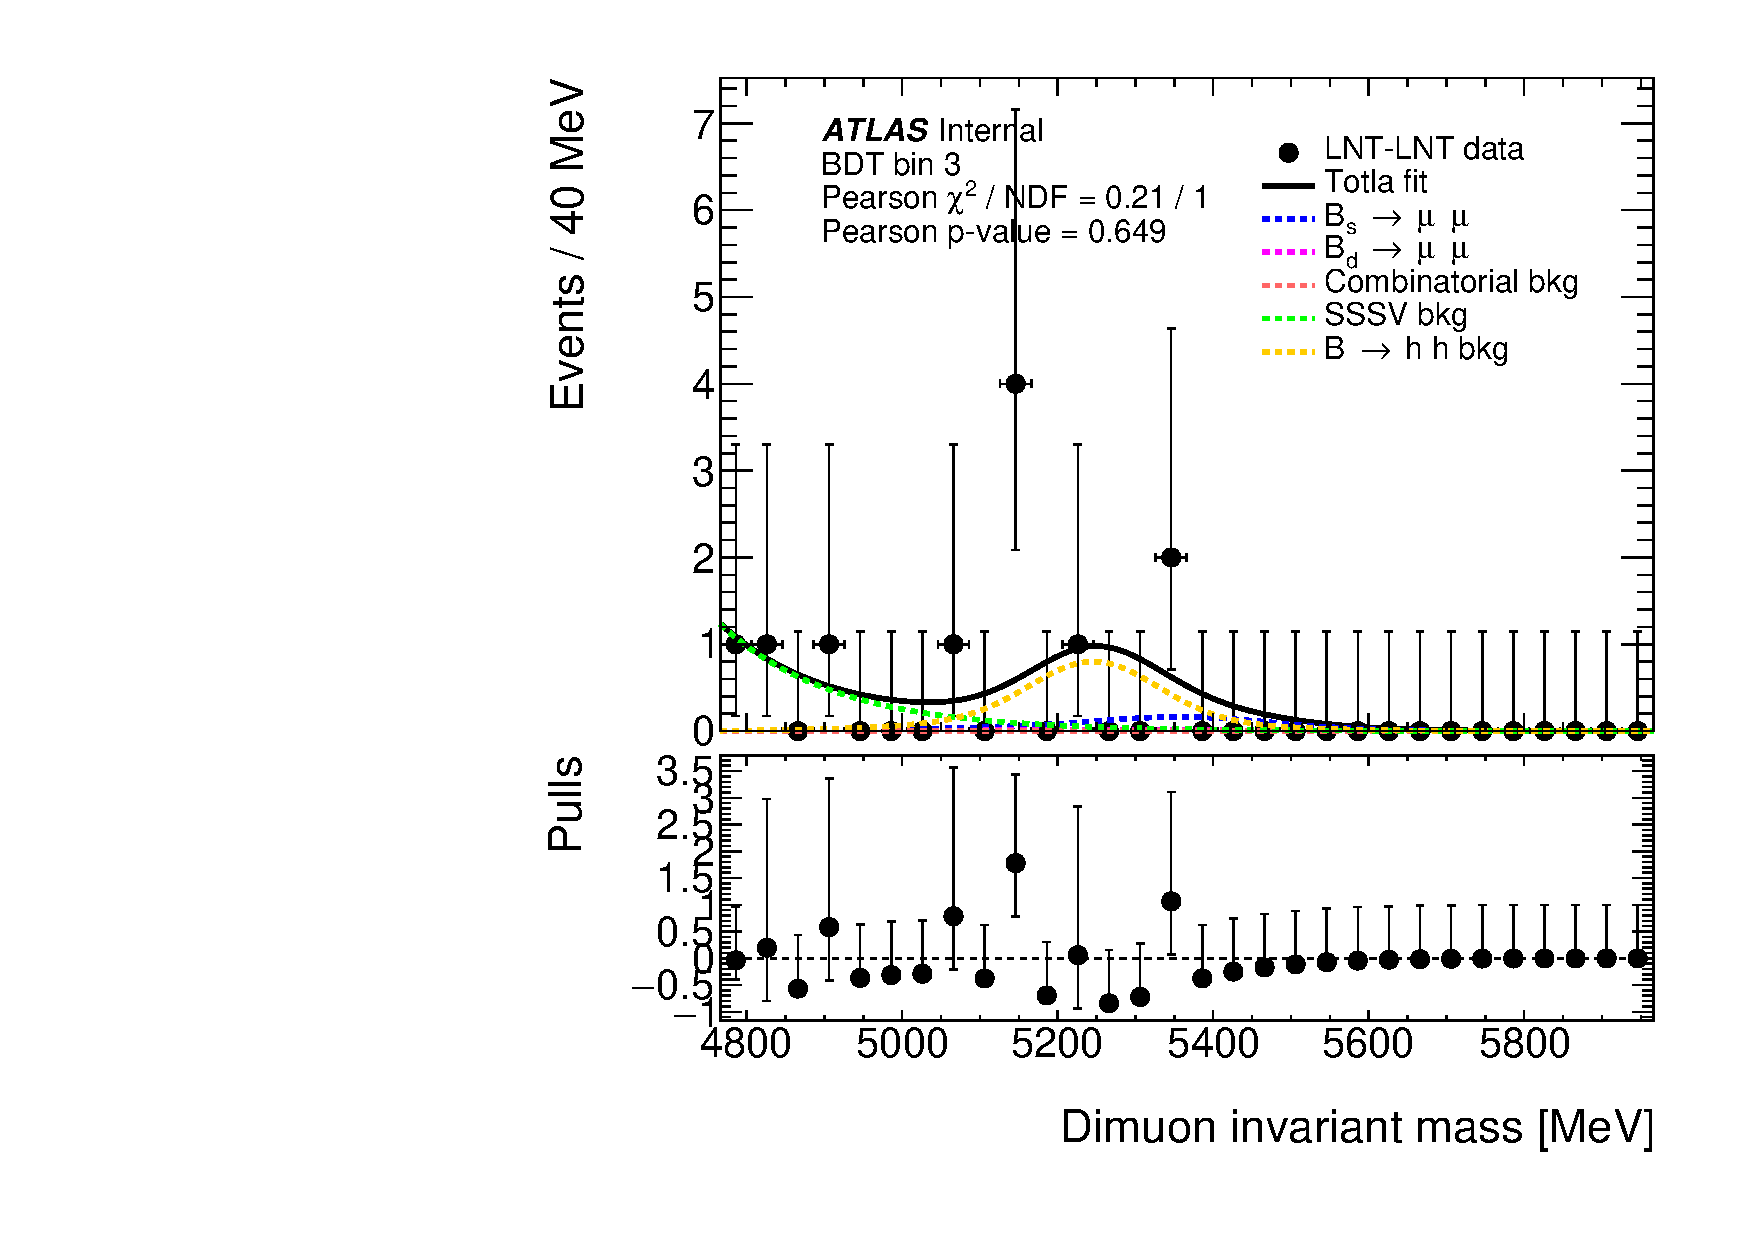
\includegraphics[width=0.5\textwidth]{figures/SignalExtraction/out_fit_Bhh_Bs_Bd_LNT-LNT_Bhh_json_all_other_T-T_nBs_nBd_fixed_pos_def_can_LNT-LNT_BDT_4_ETA_1.pdf}
    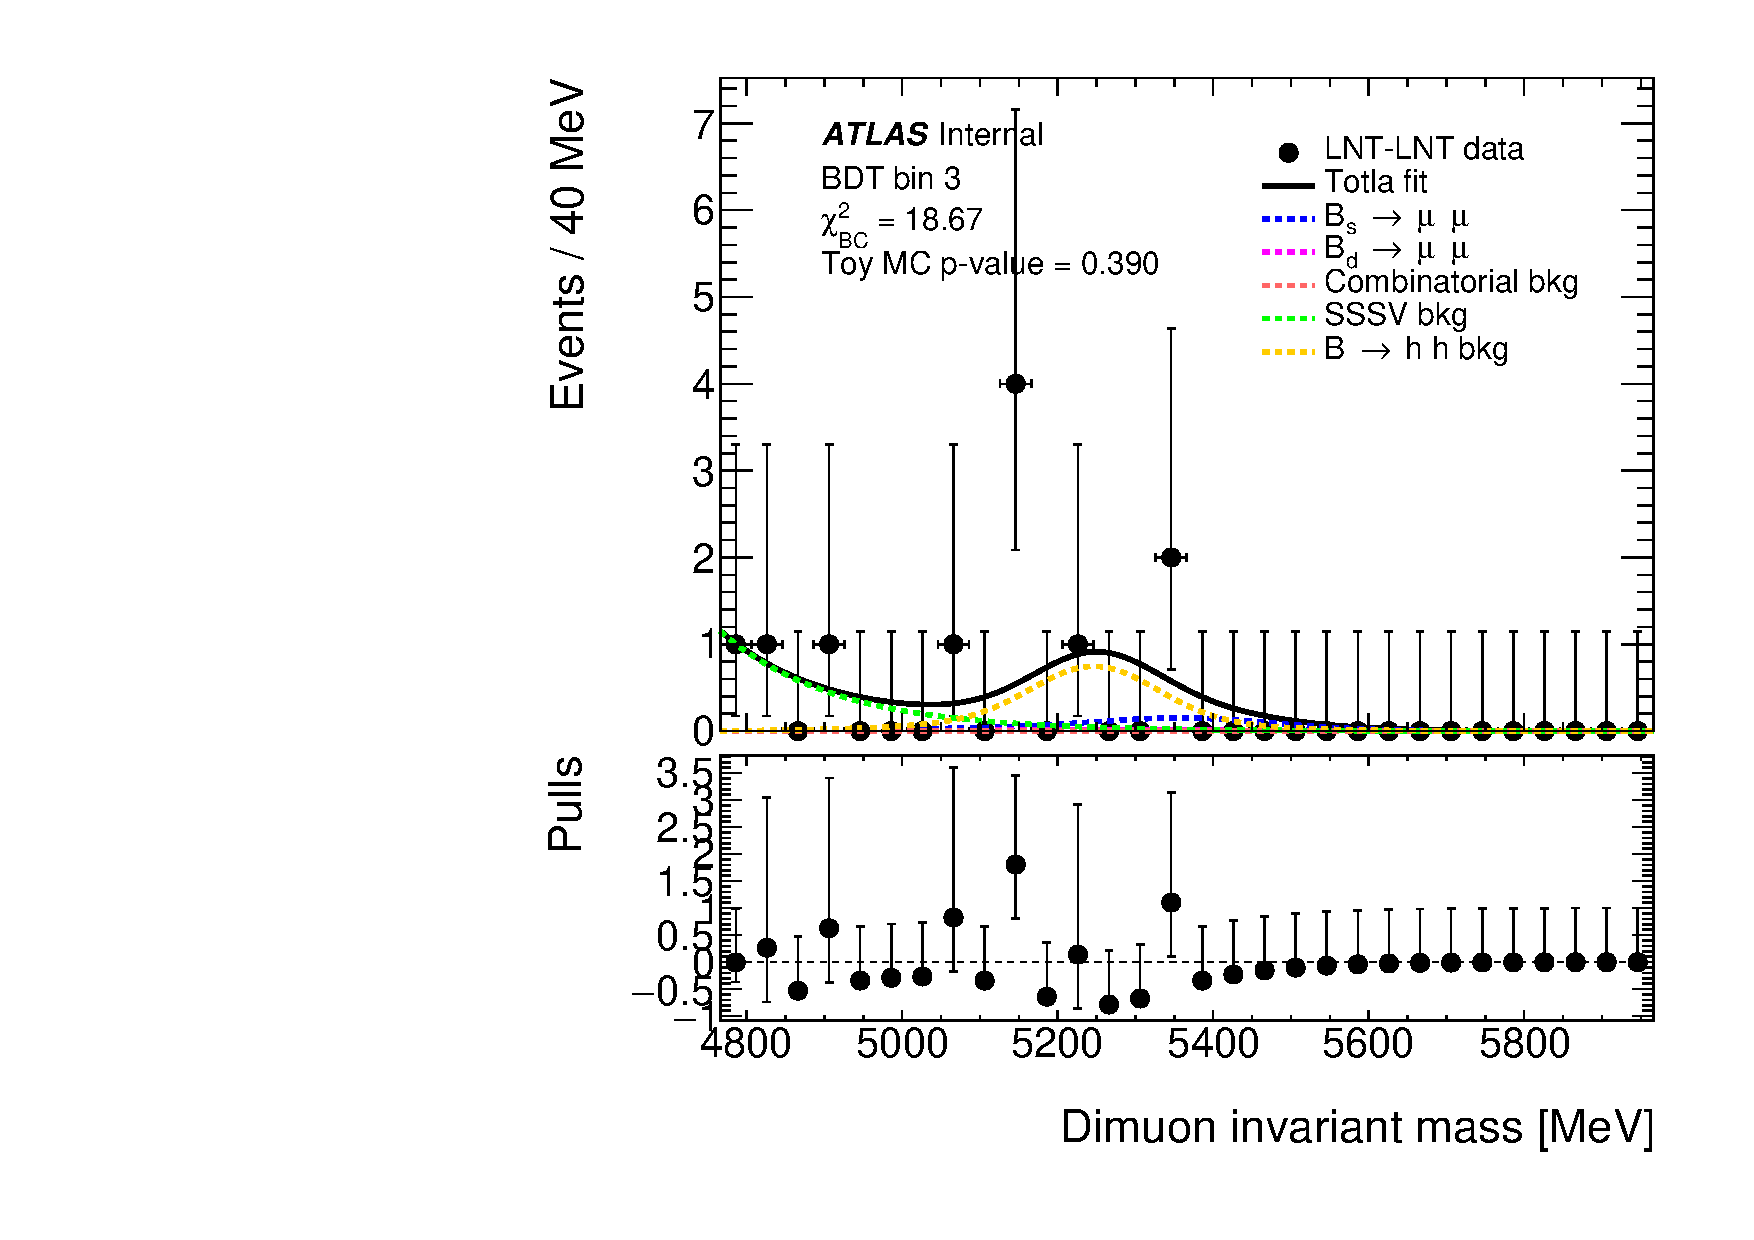
\includegraphics[width=0.5\textwidth]{figures/SignalExtraction/out_fit_Bhh_LNT_LNT_toy_MC_p_val_can_LNT-LNT_BDT_4_ETA_1.pdf}  % p-value from toy MC , BC Chi2 
    \label{fig:LNT-LNTdatafitBin3}
  }
  \caption{Unbinned extended maximum likelihood fit performed simultaneously in BDT bin 0 \protect\subref{fig:LNT-LNTdatafitBin0}, 1 \protect\subref{fig:LNT-LNTdatafitBin1}, 2 \protect\subref{fig:LNT-LNTdatafitBin2}, and 3 \protect\subref{fig:LNT-LNTdatafitBin3} on the LNT-LNT data with the adjusted baseline model as described in text. Also shown are the the Baker-Cousins $\chi^{2}$, along with the p-value obtained by the frequentist toy MC approach.} 
  \label{fig:LNT-LNTdatafit}
\end{figure}

To get a prediction in the T-T signal region to be used as a constraint on the \Bhh yield in the full baseline model intended on data, we translate the LNT-LNT data \Bhh yield into the T-T region using a ratio of counted \Bhh MC events in the full fit BDT range using all available events including those outside the mass fit range:
\begin{eqnarray}
  N_{hh'}^{T-T} = \frac{MC_{hh'}^{T-T}}{MC_{hh'}^{LNT-LNT}} \times N_{hh'}^{LNT-LNT}
  = (0.64 \pm 0.17) \times (13.4 \pm 5.5) = (8.6 \pm 4.1) \text{ events}
  \label{eq:T-T_LNT-LNT_dataBhhYield} 
\end{eqnarray}
(compared to the expectation of $13.39 \pm 0.56$ events). This data driven estimate will be used as the constraint on the \Bhh yield in the final fit.

As a loose cross-check of the procedure used to translate the LNT-LNT \Bhh yield into the T-T region we also translate the LNT-LNT \Bhh yield into the T-LNT + LNT-T region, which is then compared to the result of a direct fit to the T-LNT + LNT-T data. For the T-LNT + LNT-T data fit the \Bhh yield is constrained to the result of the LNT-LNT data \Bhh yield translated into the T-LNT + LNT-T region as a mean of assessing the compatibility of the scaled result in data. The constraint is therefore
\begin{eqnarray}
  N_{hh'}^{T-LNT+LNT-T} = \frac{MC_{hh'}^{T-LNT+LNT-T}}{MC_{hh'}^{LNT-LNT}} \times N_{hh'}^{LNT-LNT}
  = (1.46 \pm 0.31) \times (13.4 \pm 5.5) = (19.6 \pm 9.0) \text{ events}
  \label{eq:T-LNT-LNT-T_LNT-LNT_dataBhhYield} 
\end{eqnarray}

Figure~\ref{fig:T-LNT-LNT-Tdatafit} shows the result of the T-LNT + LNT-T data fit with the constraint on the \Bhh yield from equation~\ref{eq:T-LNT-LNT-T_LNT-LNT_dataBhhYield}. The fitted shape reproduces the data reasonably well with a satisfactory quality of the fit in each BDT bin. The resulting \Bhh yield was found to be $N^{T-LNT+LNT-T}_{hh'} = 8.9 \pm 7.9$ ($30.6 \pm 7.5$ expected). The MC based scaling method of data driven yield estimates into orthogonal regions is consistent for the loose cross check region, and is therefore applicable for the scaling of the $Bhh$ yield into the signal region. 
\begin{figure}[ht!]
  \centering
  \subfloat[BDT bin 0 fit with BDT boundaries at {[0.1609,0.2636]}.]{
    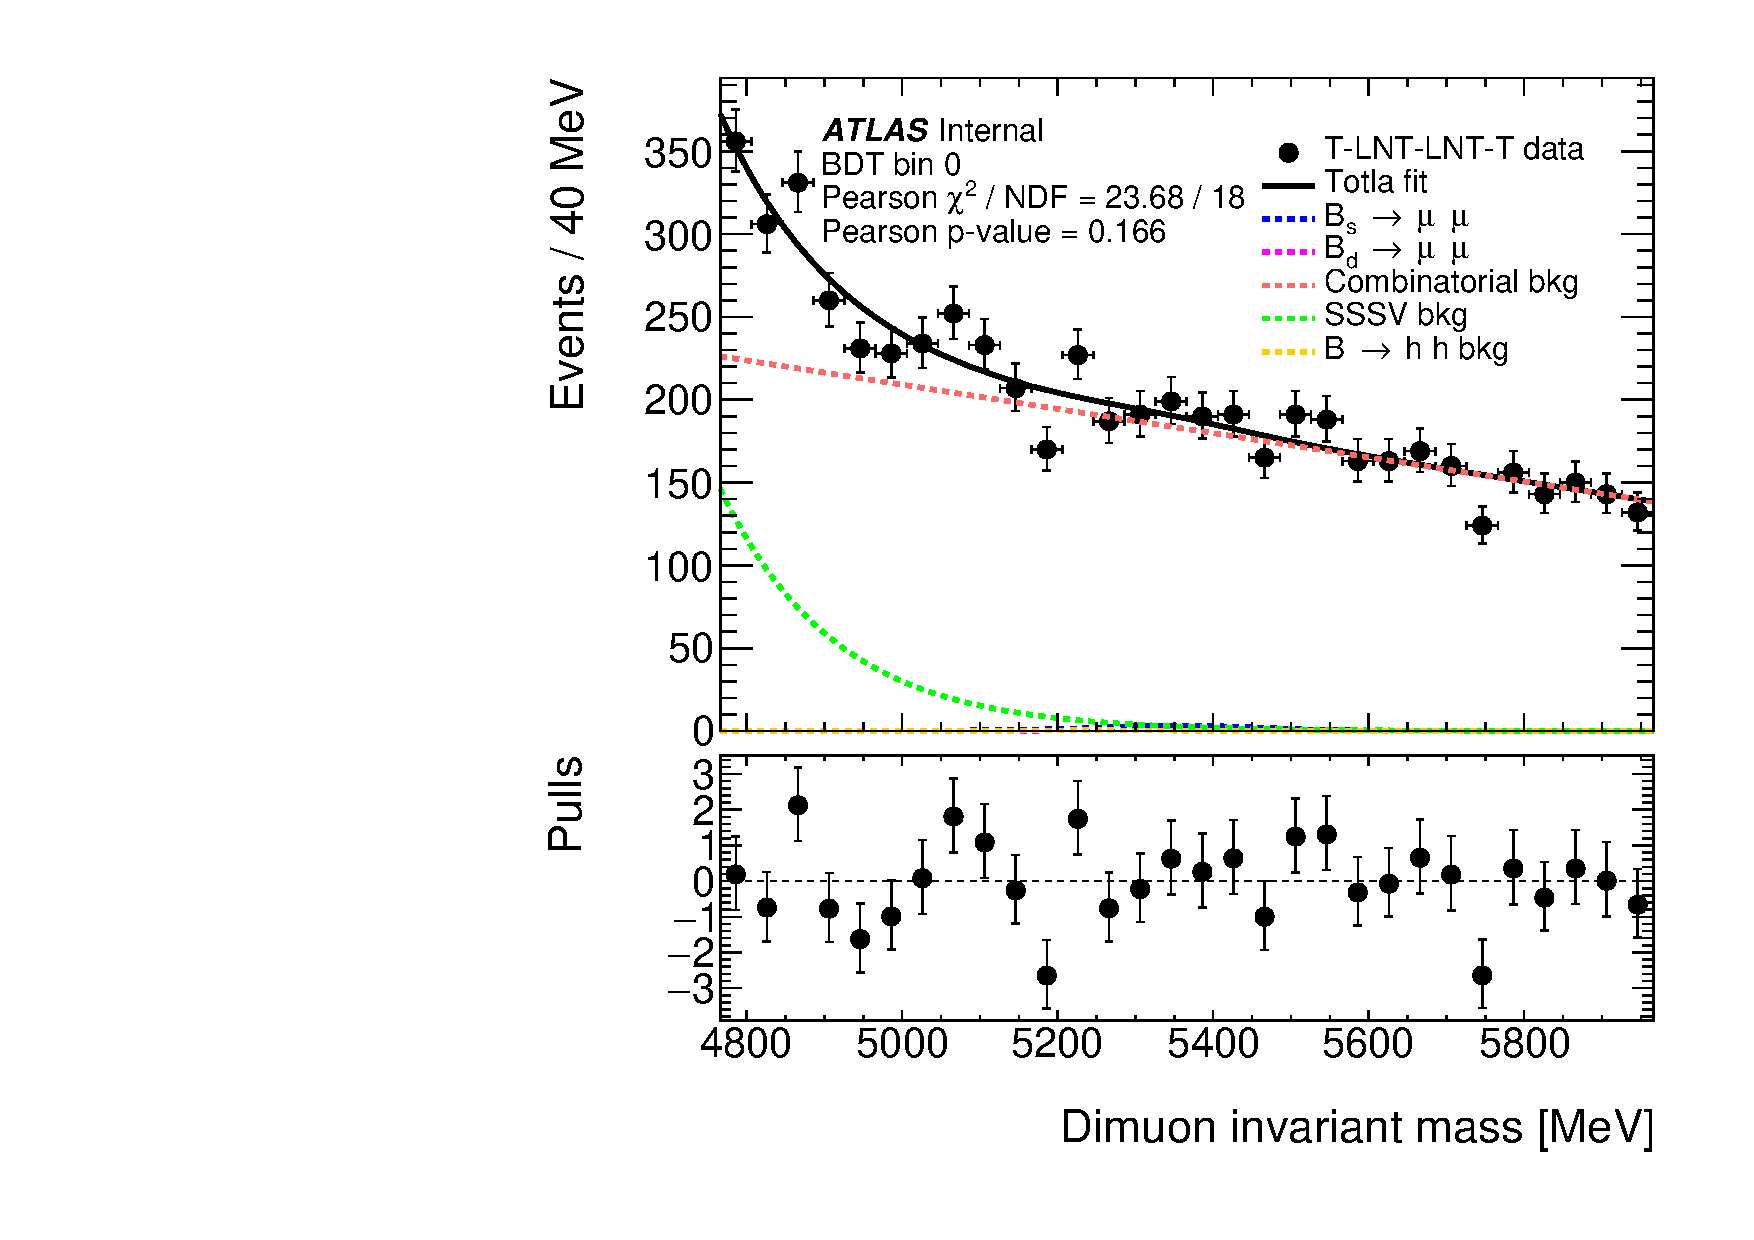
\includegraphics[width=0.5\textwidth]{figures/SignalExtraction/out_fit_Bhh_Bs_Bd_T-LNT-LNT-T_Bhh_json_all_other_T-T_nBs_nBd_fixed_nBhh_constr_LNT_LNT_pos_def_can_T-LNT-LNT-T_BDT_1_ETA_1.pdf}
    \label{fig:T-LNT-LNT-TdatafitBin0}
  }
  \subfloat[BDT bin 1 fit with BDT boundaries at {[0.2636,0.3405]}.]{
    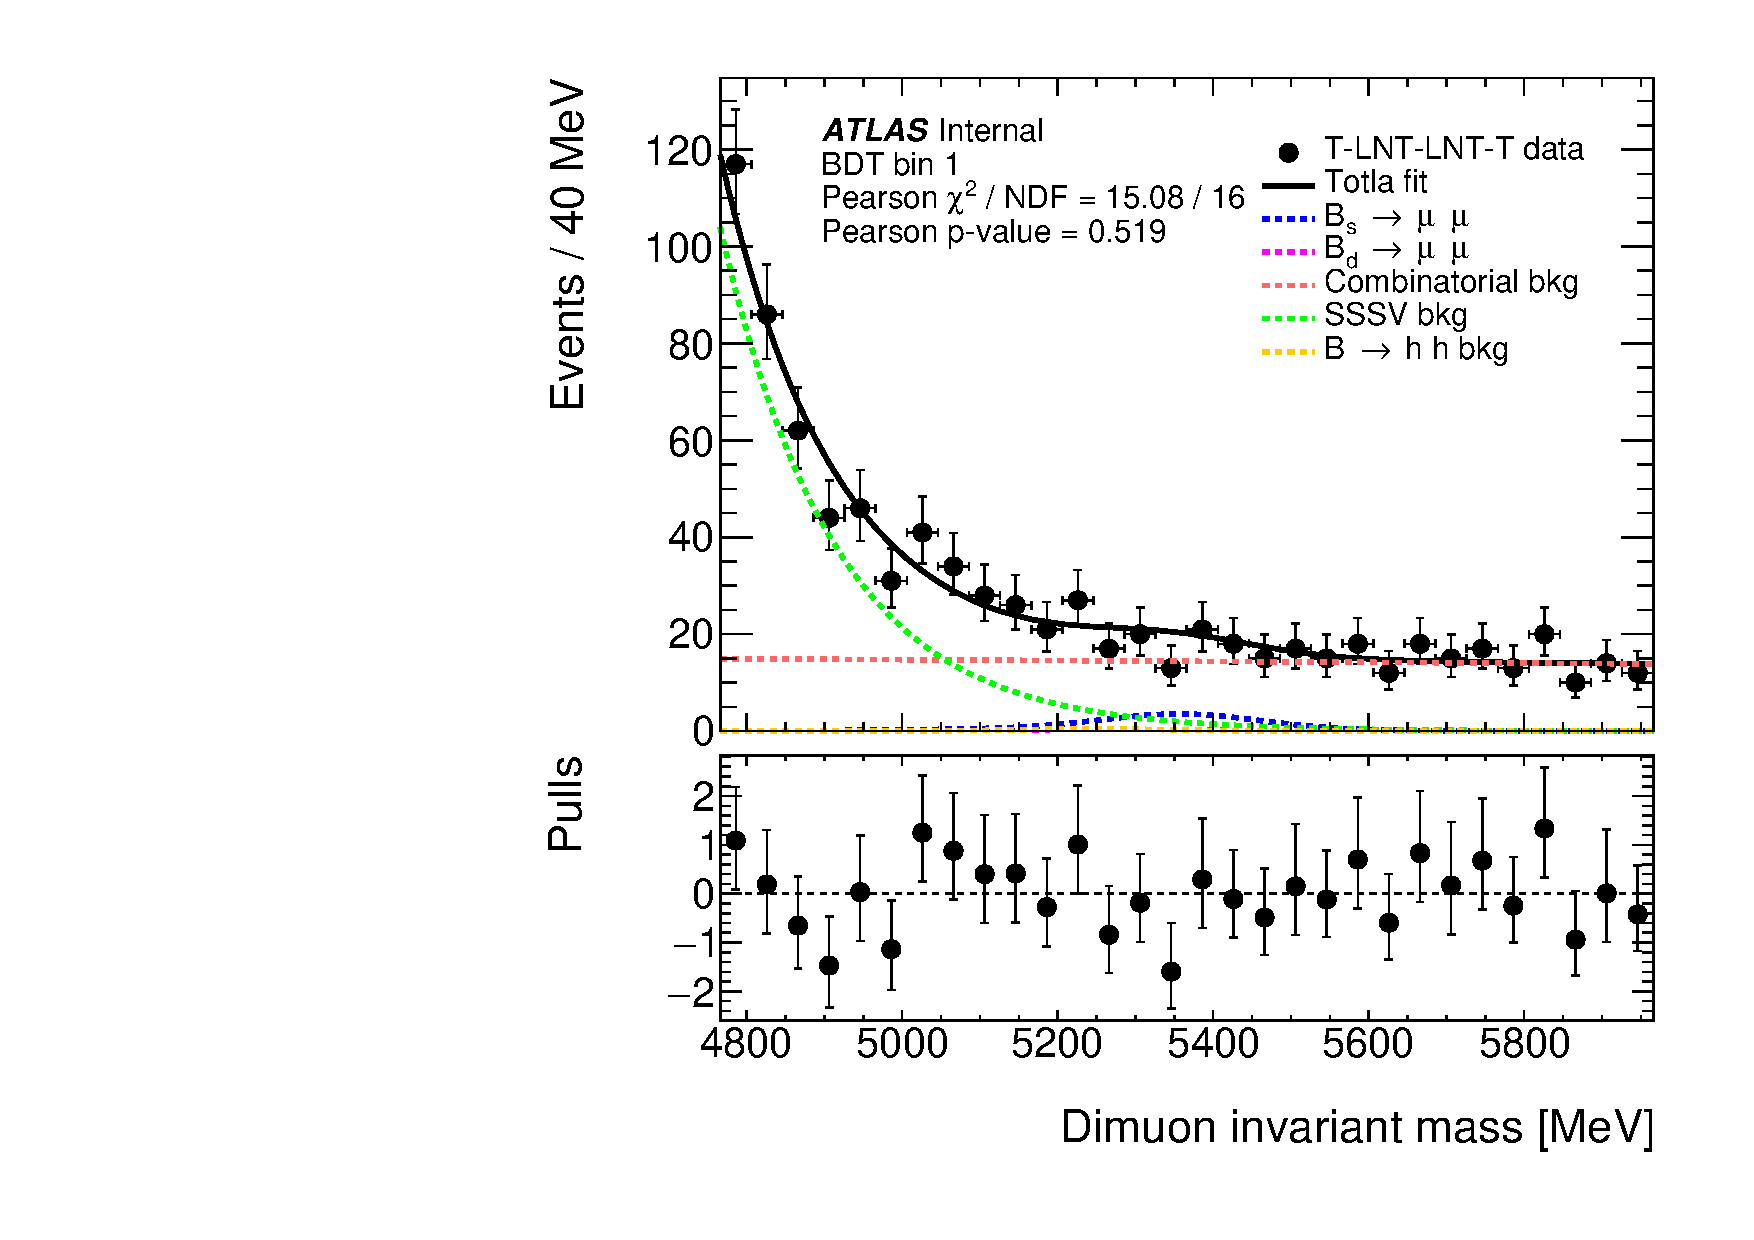
\includegraphics[width=0.5\textwidth]{figures/SignalExtraction/out_fit_Bhh_Bs_Bd_T-LNT-LNT-T_Bhh_json_all_other_T-T_nBs_nBd_fixed_nBhh_constr_LNT_LNT_pos_def_can_T-LNT-LNT-T_BDT_2_ETA_1.pdf}
    \label{fig:T-LNT-LNT-TdatafitBin1}
  }
  \\
  \subfloat[BDT bin 2 fit with BDT boundaries at {[0.3405,0.4055]}.]{
    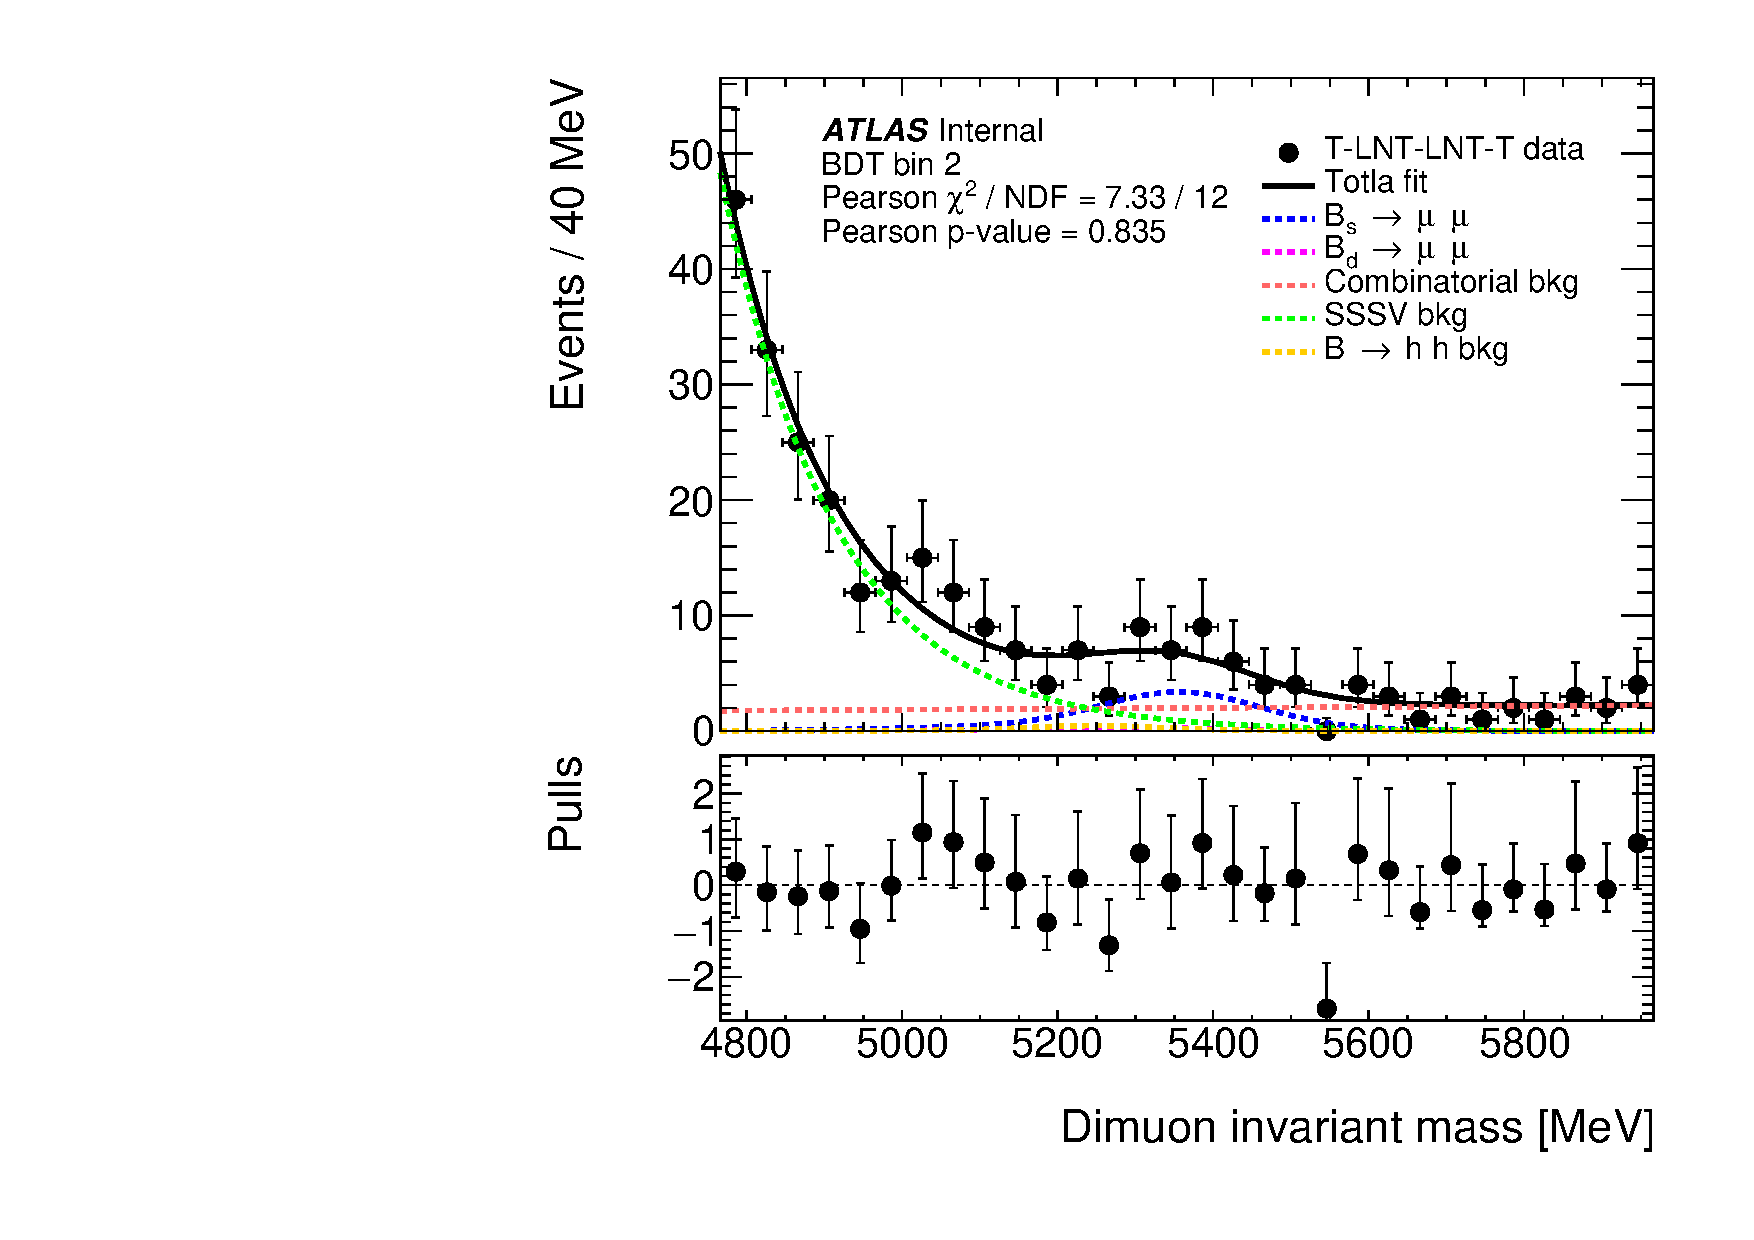
\includegraphics[width=0.5\textwidth]{figures/SignalExtraction/out_fit_Bhh_Bs_Bd_T-LNT-LNT-T_Bhh_json_all_other_T-T_nBs_nBd_fixed_nBhh_constr_LNT_LNT_pos_def_can_T-LNT-LNT-T_BDT_3_ETA_1.pdf}
    \label{fig:T-LNT-LNT-TdatafitBin2}
  }
  \subfloat[BDT bin 3 fit with BDT boundaries at {[0.4055,1.0000]}.]{
    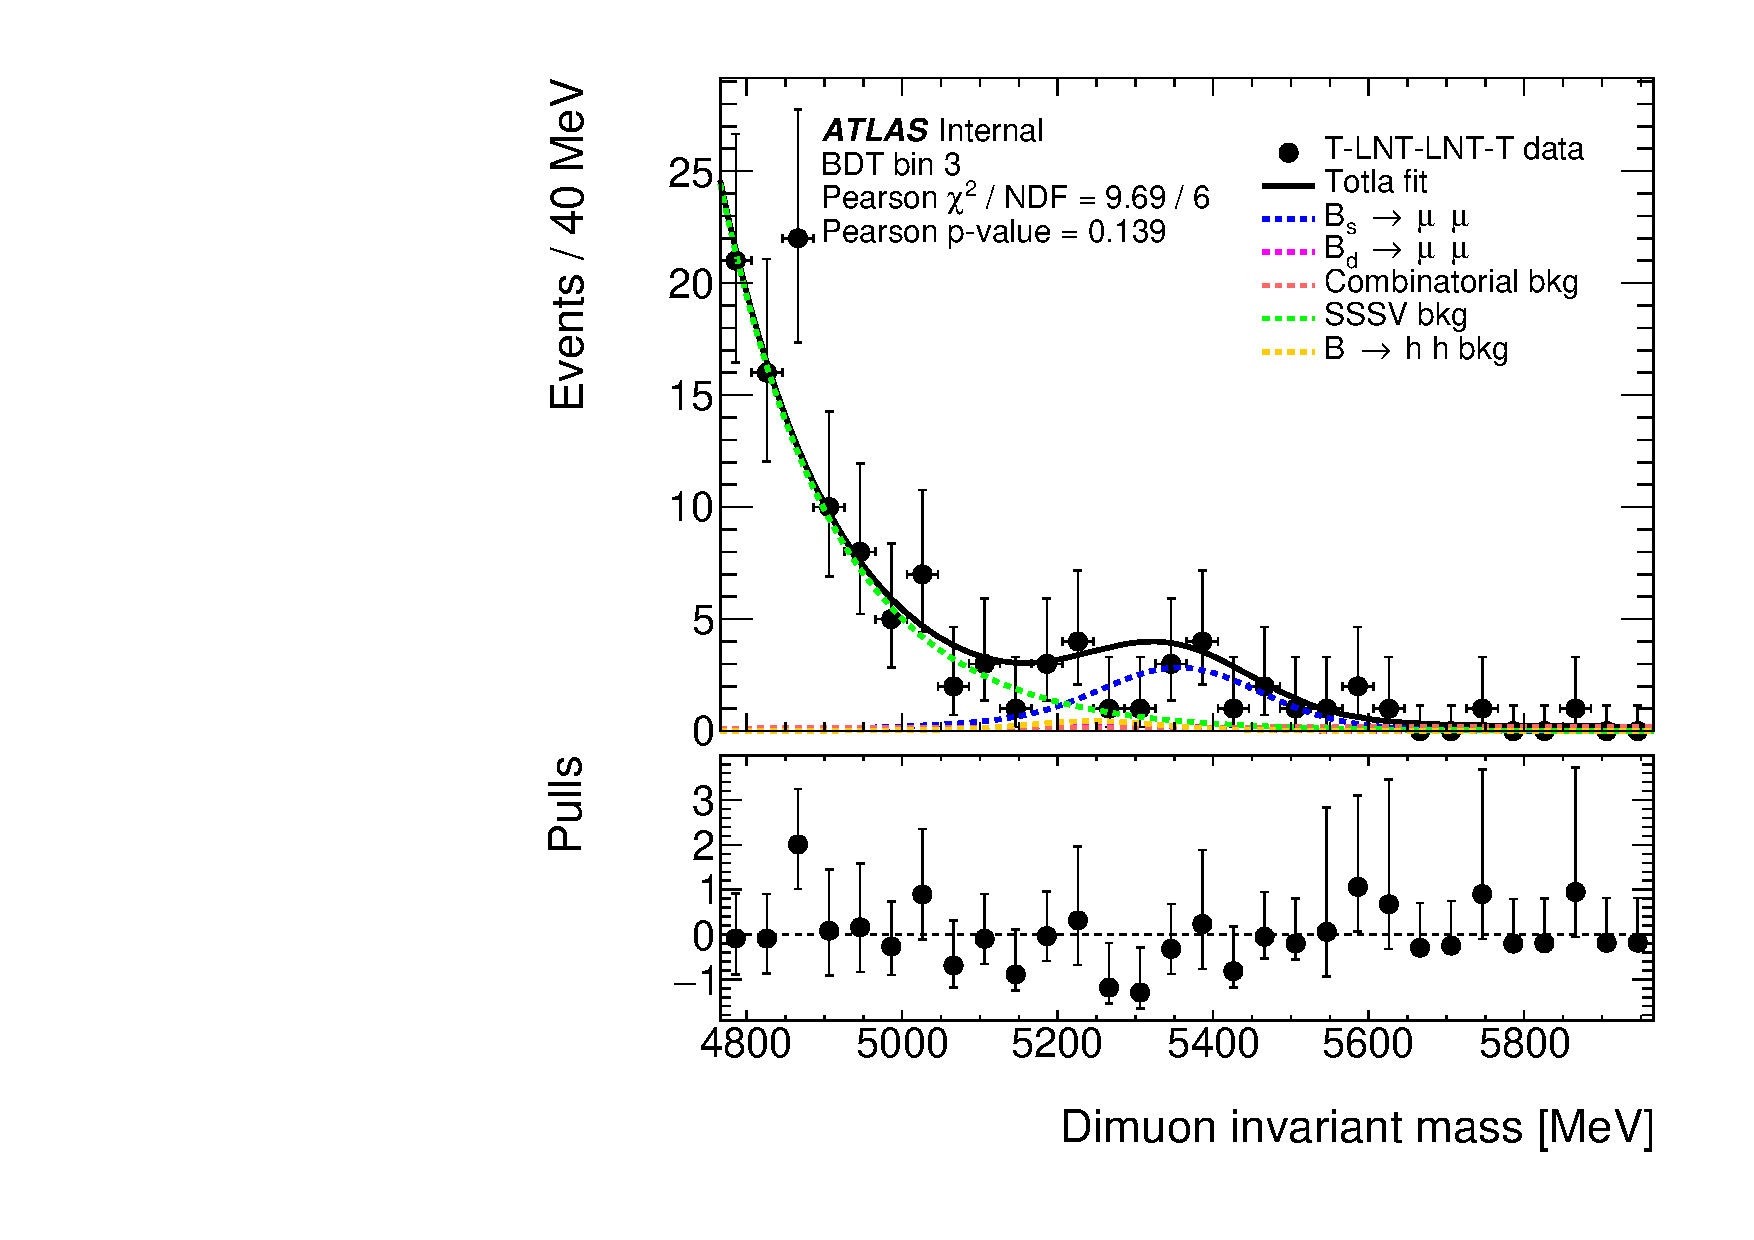
\includegraphics[width=0.5\textwidth]{figures/SignalExtraction/out_fit_Bhh_Bs_Bd_T-LNT-LNT-T_Bhh_json_all_other_T-T_nBs_nBd_fixed_nBhh_constr_LNT_LNT_pos_def_can_T-LNT-LNT-T_BDT_4_ETA_1.pdf}
    \label{fig:T-LNT-LNT-TdatafitBin3}
  }
  \caption{Unbinned extended maximum likelihood fit performed simultaneously in BDT bin 0 \protect\subref{fig:T-LNT-LNT-TdatafitBin0}, 1 \protect\subref{fig:T-LNT-LNT-TdatafitBin1}, 2 \protect\subref{fig:T-LNT-LNT-TdatafitBin2}, and 3 \protect\subref{fig:T-LNT-LNT-TdatafitBin3} on the T-LNT + LNT-T data with the adjusted baseline model as described in text and an additional constraint on the \Bhh yield from the translated LNT-LNT data fit result.} 
  \label{fig:T-LNT-LNT-Tdatafit}
\end{figure}

The ratio $\frac{N_{hh'}^{LNT-LNT}}{N_{hh'}^{T-LNT+LNT-T}} = 1.6 \pm 9.7$ measures directly the single-leg hadron species-averaged fake rate for the \Bhh daughters. From the data measurements we can can also estimate the species-averaged per-leg T vs L relative fake rate $\frac{N_{hh'}^{T-LNT+LNT-T}}{N_{hh'}^{T-LNT+LNT-T} + 2 \times N_{hh'}^{LNT-LNT}} = 0.24 \pm 0.18$. \textcolor{red}{Also all this needs to be checked over, quite large uncertainties, and not sure how useful this is to be given here.}